\documentclass[12pt,a4paper]{report}

% --- Paquets bàsics ---
\usepackage[catalan]{babel}
\usepackage[utf8]{inputenc}
\usepackage[T1]{fontenc}
\usepackage{lmodern}
\usepackage{geometry}
\usepackage{setspace}
\usepackage{graphicx}
\usepackage[hidelinks]{hyperref}
\usepackage{amsmath}
\usepackage{amsfonts}
\usepackage{amssymb}
\usepackage{float}
\usepackage{listings}
\usepackage{xcolor}
\usepackage{caption}
\usepackage{subcaption}
\lstdefinelanguage{CSharp}{
  language=[Sharp]C
}

\lstset{
  basicstyle=\ttfamily\footnotesize,
  breaklines=true,
  breakatwhitespace=false,
  postbreak=\mbox{\textcolor{red}{$\hookrightarrow$}\space},
  captionpos=b,
  frame=single,
  framerule=0.5pt,
  rulecolor=\color{gray!60},
  aboveskip=6pt,
  belowskip=6pt,
  keywordstyle=\color{blue},
  commentstyle=\color{gray},
  stringstyle=\color{teal},
  showstringspaces=false,
  tabsize=2
}



\begin{document}

\chapter{CREACIO DEL SISTEMA EN UNITY}
\section{Disseny i implementació de la planta virtual en Unity}

Una vegada definits el procés industrial i l'arquitectura de comunicació del sistema, es va procedir al desenvolupament de la planta virtual mitjançant el motor gràfic Unity.

Aquest apartat descriu les decisions de disseny preses durant la construcció dels diferents components del sistema, així com la manera en què s'han implementat els comportaments necessaris mitjançant scripts. Es farà referència als conceptes mencionats en la part de teoria de Unity (citar capitulo)

L'objectiu principal d'aquesta implementació  era reproduir el comportament d'una petita planta industrial automatitzada intentant que tot tingui un semblant realista ja sigui en l'apartat visual, en la funcionalitat del sistema i en la simplicitat de simulació.

\subsection{Construcció de l'entorn de la planta} 

Abans d'integrar els diferents elements del procés industrial, es va crear l'espai físic que representa la planta dins de Unity.

Per definir l'entorn de treball, es va construir una sala utilitzant objectes geomètrics bàsics del motor. Concretament, es van utilitzar quatre \texttt{Cube} per representar les parets, ajustant-ne la mida i posició per delimitar correctament l'espai de simulació. Per al sòl es va utilitzar un objecte \texttt{Plane}, que permet cobrir superfícies àmplies de manera eficient.

Pel que fa a la selecció dels materials, s'han tingut en compte criteris habituals en entorns industrials, com ara la resistència mecànica, la durabilitat davant del desgast, la facilitat de neteja i la seguretat (superfícies antilliscants) \cite{industrial_floor_molins,paviments_sika}.

En base a aquests criteris, els paviments industrials acostumen a utilitzar materials com el formigó polit, les resines epoxi o els paviments de poliuretà. En aquest projecte s'ha optat per una textura de \textbf{formigó polit} (Figura \ref{fig:formigo}), ja que representa de manera adequada el tipus de sòl habitual en magatzems i instal·lacions logístiques.

Pel que fa a les parets, en entorns industrials són comunes solucions com el maó, els panells metàl·lics o superfícies pintades. En aquest cas, s'ha seleccionat una textura de \textbf{maó pintat} (Figura \ref{fig:mao}), que ofereix una representació visual coherent amb una nau industrial real.

\begin{figure}[H]
\centering
\begin{subfigure}{0.3\textwidth}
    \centering
    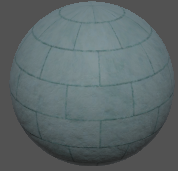
\includegraphics[width=\linewidth]{images/concrete_texture.png}
    \caption*{Textura de formigó polit \cite{texture_concrete}}
    \label{fig:formigo}
\end{subfigure}
\hspace{1cm}
\begin{subfigure}{0.3\textwidth}
    \centering
    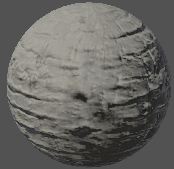
\includegraphics[width=\linewidth]{images/brick_texture.png}
    \caption*{Textura de maó pintat \cite{texture_brick}}
    \label{fig:mao}
\end{subfigure}
\caption{Materials utilitzats per a la construcció de l'entorn industrial}
\end{figure}

\subsection{Models 3D utilitzats en la planta}

La major part dels elements mecànics de la planta no han estat modelats des de zero, sinó que s'han obtingut a partir de repositoris públics d'actius per a Unity. Això ha permès centrar el desenvolupament en la lògica del sistema i el comportament dels components.

Tot i això, la majoria dels models han estat adaptats per ajustar-los a les necessitats del projecte. Principalment, s'han modificat els materials originals per aconseguir una estètica més coherent amb l'entorn industrial definit.

En alguns casos concrets, com els transelevadors, els models 3D han estat editats mitjançant \textit{Blender} \cite{blender_download} per simplificar l'estructura, separar components i adaptar-los al comportament requerit dins de la simulació. De manera similar, les estanteries també han estat ajustades a partir del model base per millorar la seva funcionalitat dins del sistema.

Els principals components utilitzats en la construcció de la planta són els següents (les imatges corresponen a la versió final utilitzada en el sistema):

\begin{itemize}

\item \textbf{Conveyor01 - Simple Rubber Conveyor}  
Model de cinta transportadora utilitzat per al transport inicial de peces dins del sistema. (Figura \ref{fig:conveyor1})

\begin{figure}[H]
    \centering
    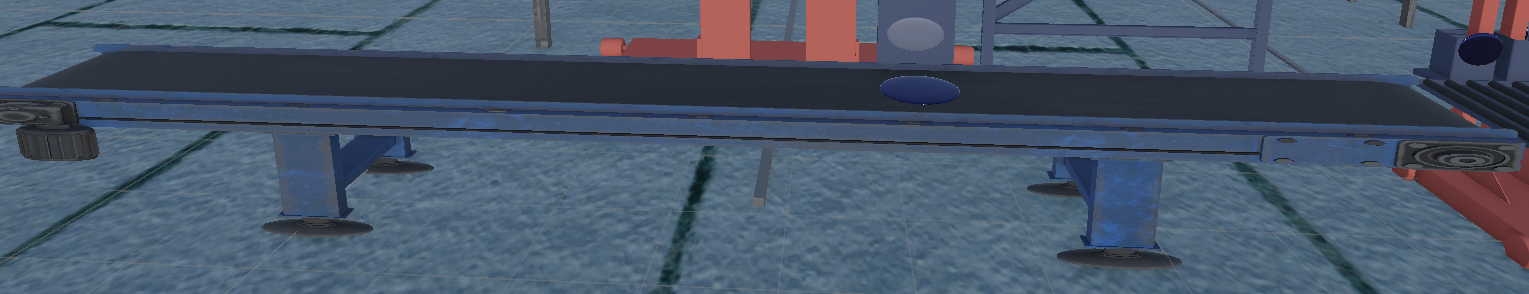
\includegraphics[width=0.7\linewidth]{images/conveyor1.png}
    \caption{Cinta principal \cite{sketchfab_conveyor}. Autor:\textit{jkvarel}}
    \label{fig:conveyor1}
\end{figure}


\item \textbf{Estanteria industrial - Warehouse Shelf Rack}  
Model utilitzat per representar les estructures d'emmagatzematge de les peces classificades dins de la planta. (Figura \ref{fig:shelf})

\begin{figure}[H]
    \centering
    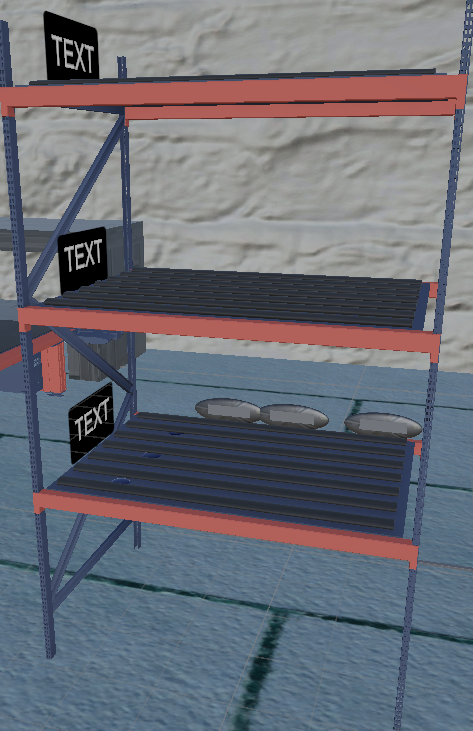
\includegraphics[width=0.4\linewidth]{images/shelf.png}
    \caption{Estanteria final, utilitzada dintre del projecte deprés d'editar per mi \cite{sketchfab_warehouse}. Autor: \textit{scailman}}
        \label{fig:shelf}

\end{figure}


\item \textbf{Cinta transportadora d'evacuació - Conveyor Belt Assembly Line}

Utilitzada en la fase final del procés per transportar les caixes fora del sistema. (Figura \ref{fig:conveyor2})

\begin{figure}[H]
    \centering
    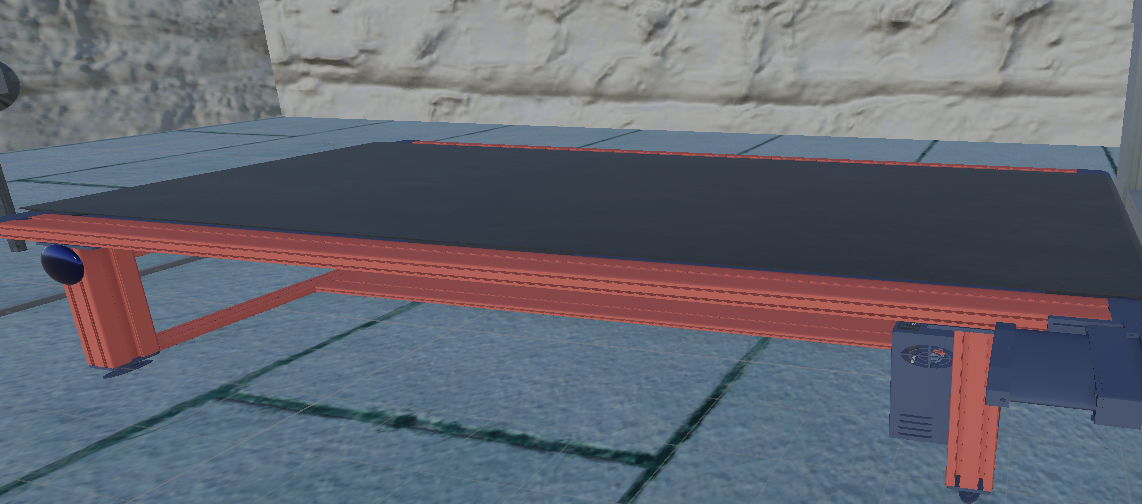
\includegraphics[width=0.5\linewidth]{images/conveyor2.png}
    \caption{Cinta evacuació \cite{conveyor_assembly}. Autor: \textit{LOVANO}}
        \label{fig:conveyor2}

\end{figure}

\item \textbf{Models de caixes - Card Boards Low Poly} 


Models utilitzats per representar les peces que circulen pel sistema de producció. (Figura \ref{fig:boxes})
\begin{figure}[H]
    \centering
    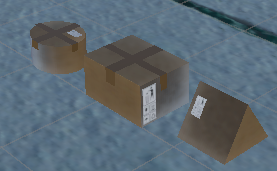
\includegraphics[width=0.35\linewidth]{images/pieces.png}
    \caption{Caixes utilitzades en el sistema \cite{boxes_model}. Autor: \textit{minitakesstudio}}
        \label{fig:boxes}

\end{figure}

\item \textbf{Transelevador - ASRS Concept}

Model utilitzat per representar el sistema automàtic d'emmagatzematge i recuperació de peces. (Figura \ref{fig:transelevadors})

\begin{figure}[H]
\centering
\begin{subfigure}{0.3\textwidth}
    \centering
    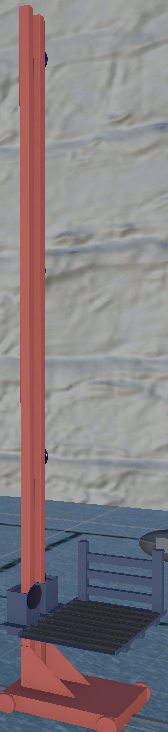
\includegraphics[width=0.4\linewidth]{images/transelevador1.png}
    \caption*{Transelevador 1}
\end{subfigure}
\hspace{1cm}
\begin{subfigure}{0.3\textwidth}
    \centering
    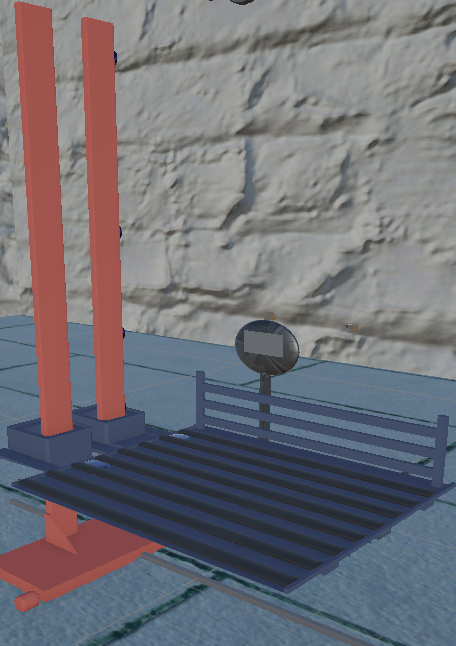
\includegraphics[width=\linewidth]{images/transelevador2.png}
    \caption*{Transelevador 2}
\end{subfigure}
\caption{Transelevador trets de la cita però utilit
zats per mi després d'editar per blender \cite{asrs_grabcad}. Autor: \textit{Ford Jacobs}}
    \label{fig:transelevadors}

\end{figure}


\item \textbf{Lamps}
Models utilitzats per representar les llums de sistema correcta i d'emergència dintre de untiy. (Figura \ref{fig:lamp})

\begin{figure}[H]
\centering
\begin{subfigure}{0.2\textwidth}
    \centering
    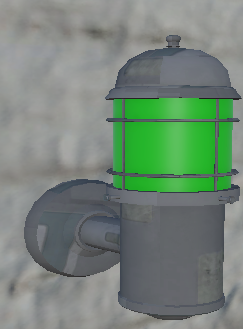
\includegraphics[width=\linewidth]{images/light_off.png}
    \caption*{Llum apagada}
\end{subfigure}
\hspace{1cm}
\begin{subfigure}{0.2\textwidth}
    \centering
    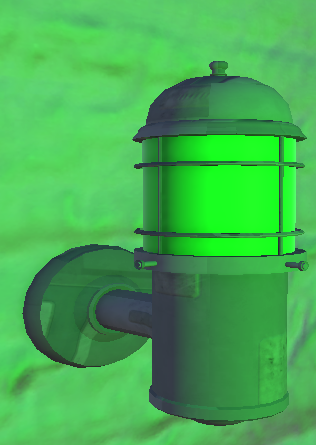
\includegraphics[width=\linewidth]{images/light_on.png}
    \caption*{Llum Encesa}
\end{subfigure}
\caption{Disseny de les làmpares i demostració de la seva funcionalitat \cite{wall_lamps}. Autor: \textit{Arrona72}.}
    \label{fig:lamp}

\end{figure}

\end{itemize}

A més dels elements anteriors, s'han implementat també sensors virtuals que permeten detectar la presència de peces en diferents punts del sistema.

\subsection{Implementació de les cintes transportadores}

Les cintes transportadores són un element clau del sistema, ja que permeten el desplaçament de les peces entre les diferents etapes del procés.

Tot i utilitzar diferents models, totes les cintes comparteixen una estructura similar. Cada model inclou una part anomenada \textbf{Belt}, que representa la superfície per on es mouen les peces i sobre la qual s'aplica el comportament funcional.


Per simular el moviment, s'han combinat dos mecanismes:

\begin{itemize}
\item \textbf{Moviment visual:} es desplaça l'\textit{offset} de la textura del material de la cinta en cada fotograma, generant la sensació de moviment continu.
\item \textbf{Moviment físic:} s'aplica una velocitat als objectes situats sobre la cinta.
\end{itemize}

\subsubsection{Configuració dels colliders}

Cada cinta disposa de dos colliders \cite{UnityColliders} amb funcions diferenciades:

\begin{itemize}
\item Un \textbf{collider estàndard}, que manté les peces recolzades sobre la superfície.
\item Un \textbf{collider tipus trigger} situat sobre el \textit{Belt}, que detecta les peces i permet aplicar el moviment.
\end{itemize}



\subsubsection{Script de moviment de la cinta}

L'script s'aplica únicament a l'objecte \textit{Belt}, permetent controlar de forma independent el comportament de la superfície.


\textit{REFERENCIAR EL SCRIPT DE BELT CONTROLLER}

Aquest script és responsable de dues funcions principals:

Aquest gestiona simultàniament:

\begin{itemize}
\item El desplaçament de la textura (dins de \textit{Update()})\cite{UnityUpdate}.
\item El moviment de les peces detectades mitjançant \textit{OnTriggerStay()}.
\end{itemize}

En primer lloc, l'efecte visual de moviment es genera mitjançant el desplaçament progressiu de la textura aplicada sobre la superfície de la cinta. Aquest càlcul es realitza dins de la funció \textit{Update()}, que s'executa en cada fotograma, modificant el paràmetre \textit{mainTextureOffset} del material. D'aquesta manera es crea la sensació de moviment continu de la cinta.

Quan una peça amb etiqueta \textit{Box} \cite{UnityTags2023} entra al trigger, s'accedeix al seu \textit{Rigidbody} \cite{UnityRigidbody} i se li aplica una velocitat en la direcció de la cinta, modificant només les components horitzontals per no afectar la gravetat.

Finalment, l'script incorpora mètodes públics per activar o desactivar la cinta i ajustar la seva velocitat, facilitant la seva integració dins de la lògica de control del sistema.

\subsection{Implementació del sistema d'estanteries}


El model 3D utilitzat per representar l'estructura d'emmagatzematge (\textit{Warehouse Shelf Rack}) no incorporava inicialment plataformes funcionals. Per aquest motiu, es va ampliar el model mitjançant la creació de nous objectes directament dins de Unity.

Concretament, per cada nivell es van afegir plataformes com a \textit{subobjectes} de l'estructura principal, facilitant així la seva gestió dins de la jerarquia.

Cada plataforma disposa d'un \textbf{Box Collider} sense \textit{Trigger}, amb la funció de suportar físicament les caixes i evitar que travessin l'estructura durant la simulació.


\begin{figure}[H]
\centering
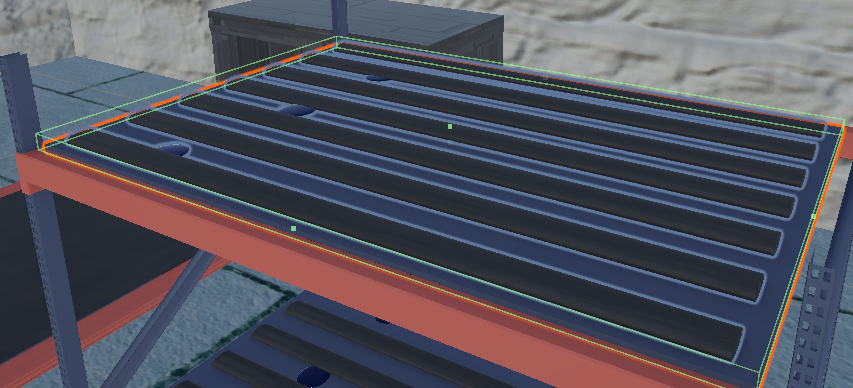
\includegraphics[width=0.7\textwidth]{images/collider_shelf.png}
\caption{Plataformes afegides a l'estanteria amb colliders}
\end{figure}

\subsubsection{Rodets de moviment dins de l'estanteria}

Addicionalment, s'ha implementat un sistema de rodets que permet reorganitzar les caixes dins de cada nivell quan una fila es completa. Aquest mecanisme desplaça les peces al llarg de la plataforma per deixar lliure la posició més propera al transelevador.

El seu funcionament és equivalent al dels rodets de la plataforma del transelevador, que es descriu amb més detall en l'apartat següent.

\subsection{Implementació del transelevador (ASRS Crane)}

El model original del sistema ASRS es trobava en format \textit{.stp}, per la qual cosa es va convertir a un format compatible amb Unity (\textit{.fbx}) \cite{stp_to_fbx}. A més a més, el model inicial presentava una estructura excessivament complexa per a la simulació, fet que va requerir la seva edició prèvia amb \textbf{Blender}. Blender permet manipular models 3D de forma més precisa que Unity quan es tracta de separar malles, dividir objectes o reorganitzar l'estructura d'un model.

 Mitjançant aquest procés es van separar els diferents components del model, especialment els rodets de la plataforma, per tal de poder controlar-los de forma independent mitjançant scripts. També es va afegir un \textit{Collider} a la plataforma per garantir el correcte suport de les peces durant el moviment.

\subsubsection{Sistema de posicionament del transelevador}

El moviment del transelevador es basa en un conjunt de posicions predefinides mitjançant \texttt{Empty GameObjects} \cite{UnityGameObjects}, col·locats en els punts on el sistema ha d'aturar-se. Aquest enfocament permet definir les posicions de forma visual dins de Unity i simplifica la configuració del moviment.

En aquest projecte:

\begin{itemize}

\item El \textbf{primer transelevador} disposa de 4 posicions horitzontals i 4 posicions verticals.

\item El \textbf{segon transelevador} disposa de 2 posicions horitzontals i 4 posicions verticals.

\end{itemize}

Cada una d'aquestes posicions correspon a una localització específica del procés industrial, com ara la cinta principal, els diferents nivells d'estanteria o la zona d'evacuació.

\subsubsection{Moviment horitzontal del transelevador}

El moviment horitzontal del transelevador es controla mitjançant un script específic que desplaça l'estructura del sistema entre les diferents posicions definides.

L'script defineix les posicions objectiu i utilitza \textit{Vector3.MoveTowards()} dins de \textit{FixedUpdate()} \cite{UnityUpdate} per desplaçar progressivament el transelevador. El moviment s'aplica mitjançant \texttt{Rigidbody.MovePosition()}, garantint una integració correcta amb el sistema físic.

\textit{CITAR SCRIPT}


\subsubsection{Moviment vertical de la plataforma}

La plataforma del transelevador disposa d'un moviment vertical \cite{UnityElevatorVideo} independent que permet posicionar la càrrega als diferents nivells de l'estanteria. 

\begin{lstlisting}[language=C]
    public Transform level0;
    ...
    void FixedUpdate()
    {
        Vector3 newLocalPos = Vector3.MoveTowards(
            transform.localPosition,
            targetLocalPosition,
            speed * Time.fixedDeltaTime
        );
        Vector3 newGlobalPos = transform.parent.TransformPoint(newLocalPos);
        rb.MovePosition(newGlobalPos);
        IsMoving = Vector3.Distance(transform.localPosition, targetLocalPosition) > 0.01f;
    }
\end{lstlisting}

En aquest cas, el moviment es calcula en coordenades locals (\textit{localPosition}) \cite{UnityTransformLocalPosition} per mantenir la coherència amb l'estructura jeràrquica del transelevador, ja que la plataforma és un objecte fill. Això evita desalineacions quan el conjunt es desplaça horitzontalment.

La nova posició es calcula amb \texttt{Vector3.MoveTowards()} i posteriorment es transforma a coordenades globals mitjançant \texttt{TransformPoint}, permetent l'ús de \texttt{Rigidbody.MovePosition()}.

El moviment s'executa dins de \texttt{FixedUpdate()}, garantint estabilitat en la simulació física. Degut a això, i al fet que el desplaçament es calcula de forma incremental, s'ha utilitzat una velocitat superior respecte al moviment horitzontal per mantenir una resposta visual coherent.

Finalment, el script incorpora la variable \textit{IsMoving}, que indica si la plataforma està en moviment. Aquesta informació és utilitzada per la lògica de control i per la seva integració amb el sistema SCADA.
\subsubsection{Sistema de rodets de la plataforma}

La plataforma del transelevador disposa d'un sistema de rodets que permet introduir o extreure les caixes. El seu funcionament és similar al d'una cinta transportadora, amb la diferència que pot operar en ambdues direccions.


\textit{CITAR SCRIPT}

L'script detecta objectes amb \textit{Rigidbody} \cite{UnityRigidbody} dins d'un collider \textit{trigger} i aplica una velocitat en la direcció definida. Aquesta direcció es pot invertir mitjançant el paràmetre \textit{forward}.

Tanmateix, per reforçar l'efecte visual, s'ha implementat un script que desplaça la textura del material dels rodets. Aquest només s'activa quan el sistema està en funcionament, mantenint coherència entre el moviment visual i físic.

\subsection{Indicadors visuals i sensors}

Per facilitar la visualització de l'estat del sistema, s'ha implementat un sistema d'indicadors visuals basat en LEDs virtuals, que reflecteixen l'estat dels sensors.

El comportament es gestiona mitjançant l'script \textit{LEDIndicator}, que canvia el material \cite{UnityMaterialsReference} de l'objecte segons l'estat del sensor associat (encès/apagat).

\begin{lstlisting}[language=C]
    public void SetActive(bool active)
    {
        if (ledRenderer == null) return;
        if (active) ledRenderer.material = onMaterial;
        else ledRenderer.material = offMaterial;
    }
\end{lstlisting}

Aquest enfocament permet desacoblar la lògica dels sensors de la seva representació visual, facilitant la reutilització del sistema.

\subsection{Tipus de sensors implementats}

S'han implementat tres tipus de sensors que simulen el comportament de dispositius industrials reals:

\begin{itemize}
\item Sensors de presència
\item Sensors òptics
\item Sensors de posició
\end{itemize}

\subsubsection{Sensors de presència}

Els sensors de presència s'utilitzen per detectar la presència de peces en punts concrets del sistema, com cintes o la plataforma del transelevador.

Es basen en un \textit{Collider} en mode \textit{Trigger}, utilitzant els esdeveniments \texttt{OnTriggerEnter} i \texttt{OnTriggerExit} per detectar l'entrada i sortida d'objectes amb etiqueta \textit{Box} \cite{UnityCollider, UnityComponents}.

Per evitar errors amb múltiples peces simultànies, s'utilitza un comptador intern en lloc de \texttt{OnTriggerStay()}, reduint també el cost computacional. Quan una peça amb etiqueta \textit{Box} entra dins del sensor, aquest activa la variable interna del sensor i encén el LED associat.

\begin{figure}[H]
\centering
\begin{subfigure}{0.2\textwidth}
    \centering
    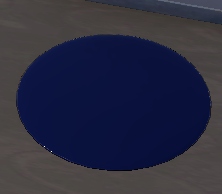
\includegraphics[width=\linewidth]{images/s1_off.png}
\end{subfigure}
\hspace{1cm}
\begin{subfigure}{0.2\textwidth}
    \centering
    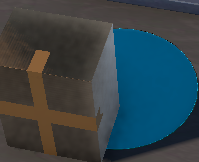
\includegraphics[width=\linewidth]{images/s1_on.png}
\end{subfigure}
\caption{Sensor de prescència apagat i encès.}
\end{figure}

\subsubsection*{Sensors òptics}

El sensor òptic permet identificar el tipus de peça mitjançant un script associat a cada objecte:

\begin{lstlisting}[language=C]
public enum PieceShape {Square, Cylinder, Triangle}
public class PieceData : MonoBehaviour
{
    public PieceShape shape;
}
\end{lstlisting}

Quan una peça entra dins del sensor, es llegeix aquesta informació i, després d'un retard controlat mitjançant un temporitzador, es valida la detecció. \textit{Citar SCRIPT}

Aquest retard simula el temps de resposta d'un sensor real i permet al sistema prendre decisions en funció del tipus de peça. Més endavant s'explica com s'ha desenvolupat aquest retard \ref{sec:timers}. 

A més de la detecció bàsica, el sistema incorpora una simulació de fallades del sensor per tal d'aproximar el comportament del model a una situació industrial real. Per aconseguir-ho, s'ha implementat una probabilitat de fallada configurable mitjançant el paràmetre \texttt{failProbability}. Cada vegada que una peça és detectada correctament i finalitza el temporitzador del sensor, es genera un valor aleatori utilitzant \texttt{Random.value}. Si aquest valor és inferior a la probabilitat configurada, el sensor no detectarà la peça, provocant que el sistema entri en estat d'avaria.

La probabilitat de fallada es pot modificar fàcilment des de l'Inspector de Unity gràcies a l'atribut:

\begin{lstlisting}[language=C]
[Range(0f, 1f)]
public float failProbability = 0.2f;
\end{lstlisting}

En aquest cas, el valor per defecte és de \texttt{0.2}, equivalent a una probabilitat de fallada del 20\%. Això permet generar situacions aleatòries d'error durant el funcionament de la simulació i comprovar la correcta resposta del sistema davant condicions no ideals.

\begin{figure}[H]
\centering
\begin{subfigure}{0.2\textwidth}
    \centering
    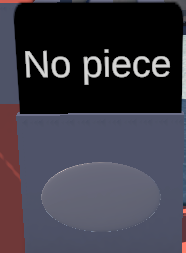
\includegraphics[width=\linewidth]{images/s2_off.png}
\end{subfigure}
\hspace{1cm}
\begin{subfigure}{0.2\textwidth}
    \centering
    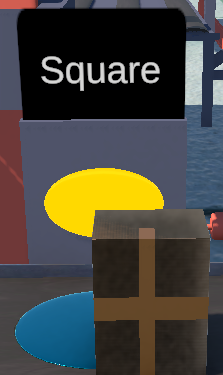
\includegraphics[width=\linewidth]{images/s2_on.png}
\end{subfigure}
\caption{Sensor òptic apagat i encès.}
\end{figure}

\subsubsection{Sensors de posició del transelevador}

Els sensors de posició determinen la ubicació del transelevador mitjançant la comparació entre la seva posició actual i posicions de referència. Es basen en la comparació entre la posició actual del transelevador i la posició objectiu en la que es troba el sensor.

Per fer aquesta comprovació es calcula la distància entre la posició actual del \textit{Rigidbody} i la posició del punt de referència corresponent.

\begin{lstlisting}[language=CSharp]
public bool Pos1 => Vector3.Distance(rb.position, position1.position) < 0.01f;
\end{lstlisting}

Quan la distància és inferior a un llindar, es considera que s'ha assolit la posició, activant també els indicadors LED associats a la vegada que s'activa la variable del sensor. Aquest sistema permet simular el comportament dels finals de carrera o sensors de posició utilitzats habitualment en sistemes AS/RS industrials.

\subsection{Sistema de llums d'estat}

S'ha implementat un sistema de llums \cite{UnityLighting} per indicar l'estat global del sistema:

\begin{itemize}
\item Verd: funcionament automàtic
\item Vermell: estat d'emergència
\item Groc: mode manual
\end{itemize}

Aquestes llums es basen en objectes \textbf{Point Light} de Unity (EXPLICAT seccio TEORIA UNITY).

El control es realitza mitjançant variables com \textit{isOk}, \textit{emergency} i \textit{manual}. L'activació es fa habilitant o deshabilitant el \textit{GameObject} a través de la funció \texttt{SetActive()}, simulant l'encesa real.

Per generar l'efecte intermitent de la llum vermella, s'utilitza un temporitzador basat en \texttt{Time.deltaTime}, que permet alternar l'estat de la llum de forma periòdica \cite{UnityTime}.

\subsection{Implementació d'un temporitzador (Timer)}
\label{sec:timers}


Per tal d'aproximar encara més el comportament del sistema a un entorn industrial real, s'ha implementat un mecanisme de temporització que permet introduir retards controlats en determinades accions del sistema.

Aquest tipus de funcionalitat és especialment important en sistemes automatitzats, ja que molts processos industrials no es realitzen de manera instantània, sinó que requereixen un temps determinat per completar-se. 

Per implementar aquesta funcionalitat s'ha desenvolupat una classe anomenada \textit{Timer}, el funcionament de la qual és equivalent a un temporitzador de tipus \textbf{TON (Timer On Delay)} utilitzat habitualment en PLCs.

El funcionament d'aquest temporitzador (CITAR SCRIPT) es basa en una entrada booleana que activa el comptatge del temps mitjançant \texttt{Time.deltaTime} \cite{UnityTime}. Quan el temps acumulat supera el valor \textit{preset}, la sortida \textit{done} esdevé \texttt{true}. Si l'entrada es desactiva abans, el temporitzador es reinicia.

\paragraph{Aplicació}

\begin{itemize}

\item \textbf{Sensor òptic:}  
Permet introduir un retard en la detecció de la peça, simulant el comportament real d'un sensor industrial que necessita un cert temps per validar la lectura. 

\item \textbf{Automatització del GRAFCET:}  
El temporitzador juga un paper fonamental en la implementació de la lògica de control basada en GRAFCET. En aquest context, els temporitzadors permeten definir transicions condicionades no només per esdeveniments (com sensors), sinó també per temps. 

\end{itemize}


\subsection{Interfície de visualització de dades (Canvas)}

A més dels indicadors LED, s'ha implementat una interfície gràfica en Unity per mostrar dades en temps real mitjançant el sistema \textit{Canvas} \cite{UnityCanvas}.

L'estructura es basa en un objecte pare \textit{GENERAL\_CANVAS} amb vuit elements fills:
\begin{itemize}
\item Quatre panells visuals
\item Quatre elements de text
\end{itemize}


\subsubsection{Visualització de comptadors}

Tres textos mostren el nombre de peces emmagatzemades. Un script (CITAR) actualitza aquest valor en cada fotograma accedint al comptador al comptador de caixes que es realitza en el procès automàtic i convertint-lo a text amb la funció \texttt{ToString()} \cite{dotnet_collections}.


\subsubsection{Visualització del sensor òptic}

El quart text mostra el tipus de peça detectada pel sensor òptic (CITAR SCRIPT). Quan no hi ha detecció es mostra \textit{"No piece"}, i en cas contrari es mostra el valor de l'enumeració \textit{PieceShape}.


\subsubsection{Ús de TextMeshPro}

S'ha utilitzat \textit{TextMeshPro} per a la representació del text, ja que ofereix millor qualitat i més flexibilitat. Els scripts treballen amb components \texttt{TMP\_Text} \cite{dotnet_text}, permetent actualitzar el contingut dinàmicament. 

Aquesta eina ofereix una qualitat de renderització de text superior en comparació amb el sistema de text tradicional, així com més opcions de personalització i control.


\subsection{Configuració de les peces del sistema}


Les peces constitueixen l'element principal que circula pel sistema industrial simulat, i per tant la seva correcta configuració és essencial per garantir un comportament físic i funcional adequat dins de l'entorn de Unity.

Cada peça disposa de l'script \textit{PieceData}, que defineix el seu tipus mitjançant una enumeració.

A nivell físic \cite{UnityRigidbody}, totes les peces comparteixen:

\begin{itemize}

\item \textbf{Component Rigidbody} amb gravetat activada

\item \textbf{Restricció de rotacions en eix X i Z} per garantir estabilitat. 

\item \textbf{Etiqueta \textit{Box}} per a la seva detecció \cite{UnityTags2023}


\end{itemize}

\subsubsection{Configuració dels colliders}

Cada tipus de peça disposa d'un sistema de col·lisió \cite{UnityColliders} adaptat a la seva geometria per tal de garantir una simulació física precisa:

\begin{itemize}

\item \textbf{Tipus A i B:} \textit{Box Collider} (eficient i adequat per formes simples)


\item \textbf{Caixa tipus C:}  \item \textbf{Tipus C:} \textit{Mesh Collider} convex per adaptar-se a la seva geometria triangular, treta del paquet \textit{ProBuilder}, amb la forma \textit{Prism}.

\end{itemize}

\subsection{Sistema de generació de peces (Spawner)}

La generació de peces dintre del sistema es realitza mitjançant l'script \textit{PieceSpawner}, integrat dins del GRAFCET, evitant una generació periòdica automàtica i permetent control total del procés.

\begin{lstlisting}[language=CSharp, caption=Script de generació de peces, label=lst:spawner]
[Range(0f,1f)] public float probC = 0.2f;
void SpawnPiece()
{
    float randomValue = Random.value;
    if (randomValue < probA) Instantiate(pieceA, transform.position, Quaternion.Euler(-90,0,0));
    else if (randomValue < probA + probB) Instantiate(pieceB, transform.position, Quaternion.identity);
    else Instantiate(pieceC, transform.position, Quaternion.identity);
 }
\end{lstlisting}


Tot i això, el sistema està preparat per fer ús dels Timers comentats previàments i fer que cada peça apareixés cada cert temps de forma controlada de forma senzilla. 


\paragraph{Selecció probabilística de peces}
El tipus de peça es determina de forma probabilística mitjançant \texttt{Random.value} i intervals acumulats definits per \texttt{probA}, \texttt{probB} i \texttt{probC}.


\paragraph{Instanciació d'objectes i gestió de rotació}

Les peces es creen amb \texttt{Instantiate()} \cite{UnityInstantiate}, definint posició i rotació inicial mitjançant \texttt{Quaternion.Euler} ((modificació de la rotació respecte el objecte original)) o \texttt{Quaternion.identity} (mateixa rotació del objecte original) \cite{UnityQuaternion}.


\subsection{Eliminació de peces del sistema}

Per tal de controlar el flux de peces dins de la planta i evitar l'acumulació infinita d'objectes en l'escena, s'ha implementat un mecanisme senzill per eliminar les peces quan arriben al final del procés.

Aquest comportament es basa en un collider configurat com a \textit{trigger} situat a la zona final de la línia de producció. Quan una peça entra en aquesta zona, és eliminada automàticament del sistema \cite{UnityLearnDestroyI}.

El codi utilitzat és el següent:

\begin{lstlisting}[language=CSharp]
using UnityEngine;

public class DestroyPiece : MonoBehaviour
{
    private void OnTriggerEnter(Collider other){
        if (other.CompareTag("Box")){
            Destroy(other.gameObject);
        }
    }
}
\end{lstlisting}

Quan una peça entra en aquesta zona, es destrueix automàticament, simulant la sortida del sistema i evitant problemes de rendiment.
\end{document}

